\documentclass[a4paper,fleqn,usenatbib]{mnras}
%=========================================================================
\usepackage{amsmath} 
\usepackage{amssymb} 
\usepackage{graphicx}
\usepackage{grffile}
\usepackage[dvips]{epsfig}
\usepackage{epsfig}  
\usepackage{color}
\usepackage{caption}
\usepackage{hyperref}
\usepackage{bm}
%Non reposionated tables
\newcommand{\HI}{{\text{H\MakeUppercase{\romannumeral 1}}} }
\newcommand{\HII}{{\text{H\MakeUppercase{\romannumeral 2}}} }
\newcommand{\lya}{\ifmmode{{\rm Ly}\alpha}\else Ly$\alpha$\ \fi}
\newcommand{\cm}{\ifmmode{{\rm cm}}\else cm\fi}
\newcommand{\ccm}{\,\mathrm{cm}^{-3}}
\newcommand{\ergps}{\,{\rm erg}\,{\rm s}\ifmmode{}^{-1}\else ${}^{-1}$\fi}
\newcommand{\Mpch}{\,{\rm Mpc}\,\ifmmode h^{-1}\else $h^{-1}$\fi}
%\newcommand{\kms}{\,\mathrm{km}\,\mathrm{s}^{-1}}
\newcommand{\dd}{\mathrm{d}}
\newcommand{\vek}[1]{\bm{#1}}
%\newcommand{\lya}{Ly$\alpha$}
\newcommand{\hb}{H$\beta$}
\newcommand{\ha}{H$\alpha$}
\newcommand{\oiii}{[OIII]}
\newcommand{\oii}{[OII]}
\newcommand{\nii}{[NII]}
\newcommand{\esca}{erg cm$^{-2}$ s$^{-1}$ \AA$^{-1}$}
\newcommand{\esc}{erg cm$^{-2}$ s$^{-1}$}
\newcommand{\es}{erg s$^{-1}$}
\newcommand{\esa}{erg s$^{-1}$}
\newcommand{\kms}{\ifmmode\mathrm{km\ s}^{-1}\else km s$^{-1}$\fi}
\newcommand{\sigmaclump}{$54.3\pm 0.6$ km s$^{-1}$}
\newcommand{\inftyclump}{$54.3\pm 5.1$ km s$^{-1}$}
\newcommand{\probaclump}{$0.96\pm 0.01$}


\begin{document}

%=========================================================================
%		FRONT MATTER
%=========================================================================
\title[Outflows and rotation in LAEs]{
Outflows and rotation in Lyman alpha emitting galaxies}
\author[M.C. Remolina-Gutierrez \& J.E. Forero-Romero]{
  Maria Camila Remolina-Guti\'errez$^1$ \&
  Jaime E. Forero-Romero $^{1}$ \thanks{je.forero@uniandes.edu.co}\\
  %%
  $^1$ Departamento de F\'isica, Universidad de los Andes, Cra. 1
  No. 18A-10 Edificio Ip, CP 111711, Bogot\'a, Colombia \\
}

\maketitle
       

\begin{abstract}
  Star-forming Compact Dwarf Galaxies (CDGs) resemble the expected
  pristine conditions of the first galaxies in the Universe and
  are the best systems to test models on primordial
galaxy formation and evolution.    
Here we report on one of such CDGs,

\end{abstract}

\begin{keywords}
galaxies: dwarf --- radiative transfer --- Methods: numerical 
\end{keywords}


%=========================================================================
%		PAPER CONTENT
%=========================================================================

%*************************************************************************

\section{Introduction}
\label{sec:intro}

Distant galaxies are key to understand early evolutionary stages of
our Universe.
Physical conditions in those galaxies allows the emergence of
Lyman-$\alpha$ line emission at $1216$ \AA \cite{PartrigePeebles}.
Galaxies detected through its Lyman-$\alpha$ emission receive the name of
spectra at  and named Lyman Alpha Emitters (LAEs).

Currently LAEs are commonly targetted in wide area galaxy surveys.
They have been effectively used to study galaxy evolution,
cosmology and the thermal history of the Universe.
This has been able through the study of their spatial distribution and
the shape of the \lya emission line.

Recent imptovements in instrumentation have revolutionized the kind of
studies that can be performed on LAEs.  
It is now possible to infer detailed kinematic maps for nearby galaxies.
The study of these maps would allow us to build data-driven models to
interpret the \lya spectra of unresolved galaxies, helping us to
constrain the physical conditions of the interstellar medium (ISM)
processing the \lya radiation.

On the ISM's features that plays an important role in shaping the \lya
is HI kinematics. 
In a static HI medium the \lya line has  two equal and symmetric peaks
around the natural \lya wavelength and zero intensity at the line's
center.
For an outflowing ISM, the line becomes
asymmetrical with a more pronounced read peak.
If the galaxy rotates, the line shows different amounts of Doppler
shifts modifying the overall line profile \cite{Garavito14}.

In this paper we present for the first time a study of the joint
effects of galaxy outflows and rotation.
We study a simplified geometrical configuration corresponding to an
spherical gas cloud with symmetrical radial outflows and a rotation
profile corresponding to a solid body.
We base our modelling on a Monte-Carlo radiative transfer code called
CLARA (Code for Lyman Alpha Radiation Analysis) presented for the
first time in \cite{CLARA}.
Besides modelling the impact of joint rotation and outflows, we also
want to check to what extent the analytical model presented by
\cite{Garavito14} to explain the effects of rotation can also be
applied in our case.

In this paper we introduce first our theoretical tools and assumptions
in Section \ref{sec:theory}, then we present the numerical results and
comparisons against the analytical solution in \ref{sec:results}.
In Section \ref{sec:discussion} we discuss our results and their
possible implications for observational analysis to finally present
our conclusions in Section \ref{sec:conclusions}.


\section{Theoretical Models}
\label{sec:theory}

\subsection{Monte-Carlo Radiative Transfer Model}

CLARA follows the propagation of individual photons through a neutral
Hydrogen medium characterized by its temperature, velocity field and
global optical depth.
The code assumes an homogeneous density throughout the simulated
volume.
In the current implementation we neglect the influence of dust.
Our basic models is an spherical distribution of neutral hydrogen,
an approximation commonly used in the literature, as it explains a
wide variety of observational features \citep{Ahn03,Verhamme06,Dijkstra06}.


The central element in this paper is the velocity field that captures
outflows and rotation.
Outflows are captured by a Hubble-like radial velocity profile with
the velocity magnitude increasing linearly with the radial
coordinate; the outflow model is fully characterized by $V_{\rm out}$, the
velocity at the sphere's surface.
Rotation follows a solid body rotation profile, which is fully
characterized by $V_{\rm rot}$, the linear velocity at the sphere's surface.

The total velocity field corresponds to the superposition of rotation and
outflows.
The cartesian components take the form

\begin{equation}
	v_{x}=\frac{x}{R}V_{\rm out}-\frac{y}{R}V_{\rm rot} ,
	\label{eq:vx}
\end{equation}

\begin{equation}
	v_{y}=\frac{y}{R}V_{\rm out}+\frac{x}{R}V_{\rm rot} ,
	\label{eq:vy}
\end{equation}

\begin{equation}
	v_{z}=\frac{z}{R}V_{\rm out},
	\label{eq:vz}
\end{equation}
%
where $x$, $y$ and $z$ are the cartesian position coordinates with the
origin at the sphere's center $R$ is the radius of the sphere and the
direction of the angular velocity vector corresponds to the $\hat{k}$
unit vector. 

For each model setup we follow $10^5$ individual photons generated at
the center of the sphere at the \lya\ line's center as they propagate
through the spere and finally scape.
We store the final frequency and propagation direction for each photon
at its last scattering.  



In Table \ref{tab:values} we list the combination of $\tau_{\rm{H}}$,
$v_{rot}$ and $v_{out}$ values used in this paper.
The range of values have some overlap with the expectations from a dwarf
galaxy with a total neutral hydrogen mass of $10^8$-$10^9$ $M_{\odot}$.
We run a total of $24$ different models.


\begin{table}[htbp]
  \begin{center}
    \begin{tabular}{|c|c|c|}
      \hline
      $\tau_{\mathrm{H}}$ & $v_{rot}$ (\kms) & $v_{out}$ (\kms) \\
      \hline
      $10^5$  & \{0\} & \{5, 25, 50\} \\
      $10^6$ & \{0\} & \{5, 25, 50\}\\
      $10^7$ & \{0\} & \{5, 25, 50\}\\
      $10^5$  & \{50, 100\} & \{25, 50, 75\} \\
      $10^6$ & \{50, 100\} & \{25, 50,75\}\\
      $10^7$ & \{50, 100\} & \{25, 50,75\}\\
      \hline    
    \end{tabular}
  \end{center}
  \caption{\textbf{Parameters' Values.} List of values that were used
    to construct the radiative transfer models. Values in braces
    for a row indicate that all possible combinations in of
    $\tau_{\rm{H}}$,
    $v_{rot}$ and $v_{out}$ are used.}
  \label{tab:values}
\end{table}


\subsection{Analytical Model for Bulk Rotation}


Rotation induces two main effects on the \lya line morphology.
First. Break of spherical symmetry due to the 
  preferential direction introduced by the rotation axis.
  This symmetry break is reflected in the observed spectra as a
  dependency on the viewing angle, $\theta$, between the line of sight
  of a distant observer and the rotaional velocity.    
Second. Line blurring as the rotational velocity increases.
  At a fixed viewing angle, faster rotation induces makes the observed
  line wider and increases the flux around the line's center. 

  
\cite{Garavito14} presented in the Appendix an analytical model that
accounts for these two features.
The basic assumption of the analytical model is that each
differential surface element on the sphere Doppler shifts the photons
that it emmits.
In this paper we introduce this ansatz by postprocessing the results
of the outflow simulations without rotation.
This allows us to produce new \lya spectra and compare them with the
full radiative transfer solution including both outflows and
rotation. 


\section{Results}
\label{sec:results}

\subsection{Monte-Carlo Radiative Transfer Model}

We evaluate first the effects of increasing rotational
velocity at fixed values of the optical depth and outflow velocity.
Figure \ref{fig:varying_rotation} summarizes the information.
All plots correspond to the same outflow velocity of $v_{out}=50$\kms,
rows have constant optical depth and columns have constant rotational
velocity.
Each panel shows different morphologies corresponding to varying
line-of-sight viewing angle.

% Esta figura deberia tener 3 x 3 vinetas. vout=50.
% cada panel tiene una curva para theta=0, 45, 90.
% |tau=1E5, vrot=0, | tau=1E5, vrot=50, | tau=1E5, vrot=100, 
% |tau=1E6, vrot=0, | tau=1E6, vrot=50, | tau=1E6, vrot=100, 
% |tau=1E7, vrot=0, | tau=1E7, vrot=50, | tau=1E7, vrot=100, 


We now evaluate the effects of increasing outflow velocity at fixed
values for the optical depth and rotational velocity.
Figure \ref{fig:varying_outflow} summarizes the information following
the same patters as Figure \ref{fig:varying_rotation}, only that this
time all plots correspond to the same rotation velocity of
$v_{rot}=50$\kms,


% Esta figura deberia tener 3 x 3 vinetas. vrot=50.
% cada panel tiene una curva para theta=0, 45, 90.
% |tau=1E5, vout=25, | tau=1E5, vout=50, | tau=1E5, vout=75,
% |tau=1E6, vout=25, | tau=1E6, vout=50, | tau=1E6, vout=75,
% |tau=1E7, vout=25, | tau=1E7, vout=50, | tau=1E7, vout=75, 



\subsection{Analytical Model for Bulk Rotation}

\section{Discussion}
\label{sec:discussion}

\subsection{Theoretical Insights}

\subsection{Observational Perspectives}

\section{Conclusions}
\label{sec:conclusions}

\bibliographystyle{mnras}
\bibliography{references}

\end{document}


\cite{DjorgovskiThompson}, \cite{Rhoads00},
\cite{Gawiser2007}, \cite{Koehler2007}, \cite{Ouchi08},
\cite{Yamada2012}, \cite{Schenker2012}, \cite{Kulas12},
\cite{Yamada2012}, \cite{Chonis2013}, \cite{Finkelstein2013},
\cite{Ostlin14}, \cite{Hayes2014}, \cite{Faisst2014},
\cite{Fumagalli2015}.
 

\section{A new LAE model}
\label{sec:newmodel}


(\cite{Adams72}, \cite{Harrington73}, \cit
e{Neufeld90}, \cite{Dijkstra06}, \cite{Verhamme06}, \cite{Forero12},
\cite{Martin2015}, \cite{Garavito14}, \cite{Neufeld91},
\cite{Laursen09}, \cite{Barnes11}, \cite{Verhamme12},
\cite{Yajima12}).\\ 


\subsection{Galaxy's Viewing Angle}

We illustrate this in
Fig. \ref{fig:model}. \\ 

\begin{figure}[h!]
  \begin{center}
    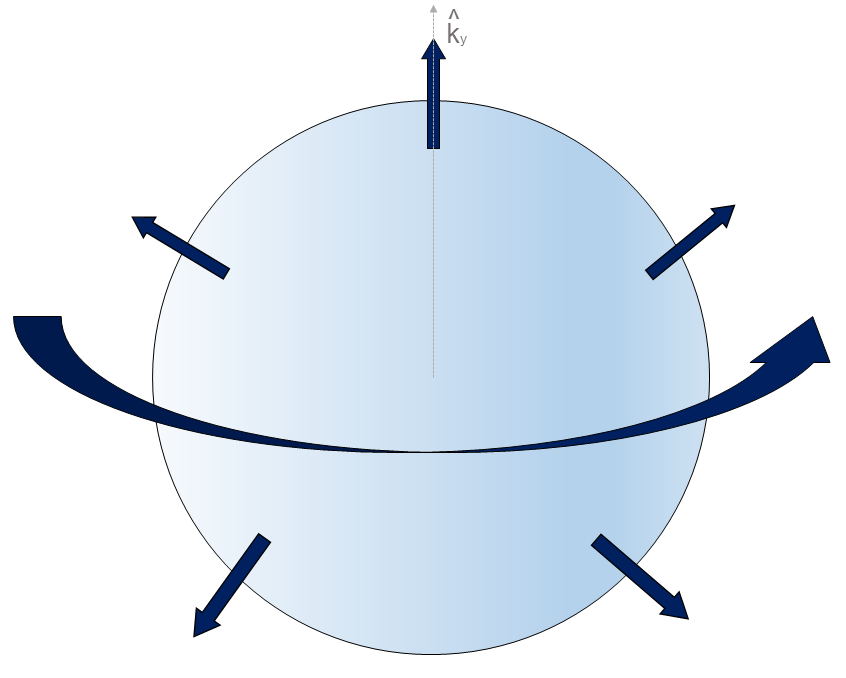
\includegraphics[width=0.48\textwidth]{./figures/model}
  \end{center}
	\caption{\textbf{Model:} Spherical LAE with tangential and radial velocities due to rotation and outflows, respectively. The galaxy cut is in the $y-z$ plane perspective. The observer is located at an specific viewing angle of the sphere. Only photons with a direction that enters in this range of vision are taken into account to build the observed spectrum.
		\label{fig:model}}
\end{figure}


\section{Results}
\label{sec:results}

\subsection{Resulting simulated spectra}
In order to define the ranges of tauh, vrot and vout, it is necessary
to refer to observational constraints. The common values for typical
LAEs that were set as parameters are in Tab. \ref{tab:values}. We run
CLARA's modified version for all the permutations of these 3
parameters. \\ 



The behavior of the resulting sets of spectra can be summarized by
Fig. \ref{fig:summary}. We concluded from the simulations a clear
creation of two asymmetric peaks around $V=0$ \kms with the tallest
peak always redshifted. We detected a strong dependence on the outflow
velocity that induces the peak asymmetry. We also detected that the
rotation velocity broadens the line horizontally. Both these effects
have been previously reported separately in the literature, so these
results can valid their superposition to some extend. \\ 

\begin{figure}[h!]
	\begin{center}
		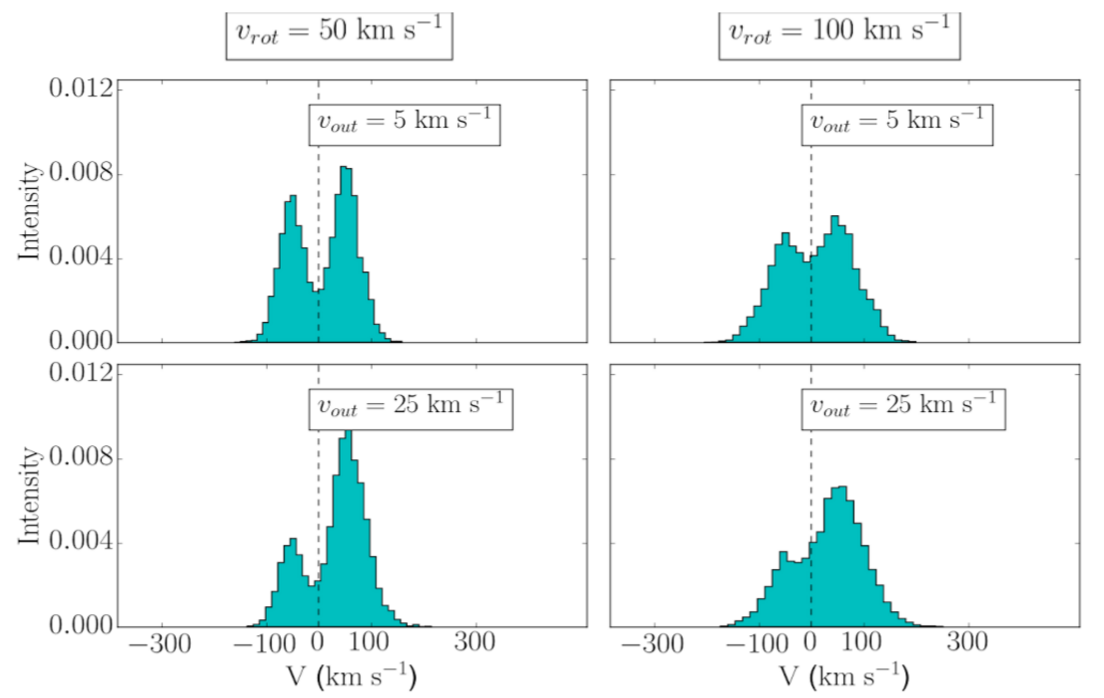
\includegraphics[width=0.48\textwidth]{./figures/summary}
	\end{center}
	\caption{\textbf{4 different \lya profiles:} With tauh$=10^5$ and $\theta \simeq 90^\circ$. The rotational velocity vrot increases to the right and the outflows velocity vout increases downwards. The intensity is in arbitrary units.
		\label{fig:summary}}
\end{figure}

\subsection{Influence of the viewing angle $\theta$}
We take now into account the viewing angle of the galaxy to build the observed spectra. For all of the physical parameters' combinations, the effect of $\theta$ in the \lya line is always the same.\\

\begin{figure}[h!]
	\begin{center}
		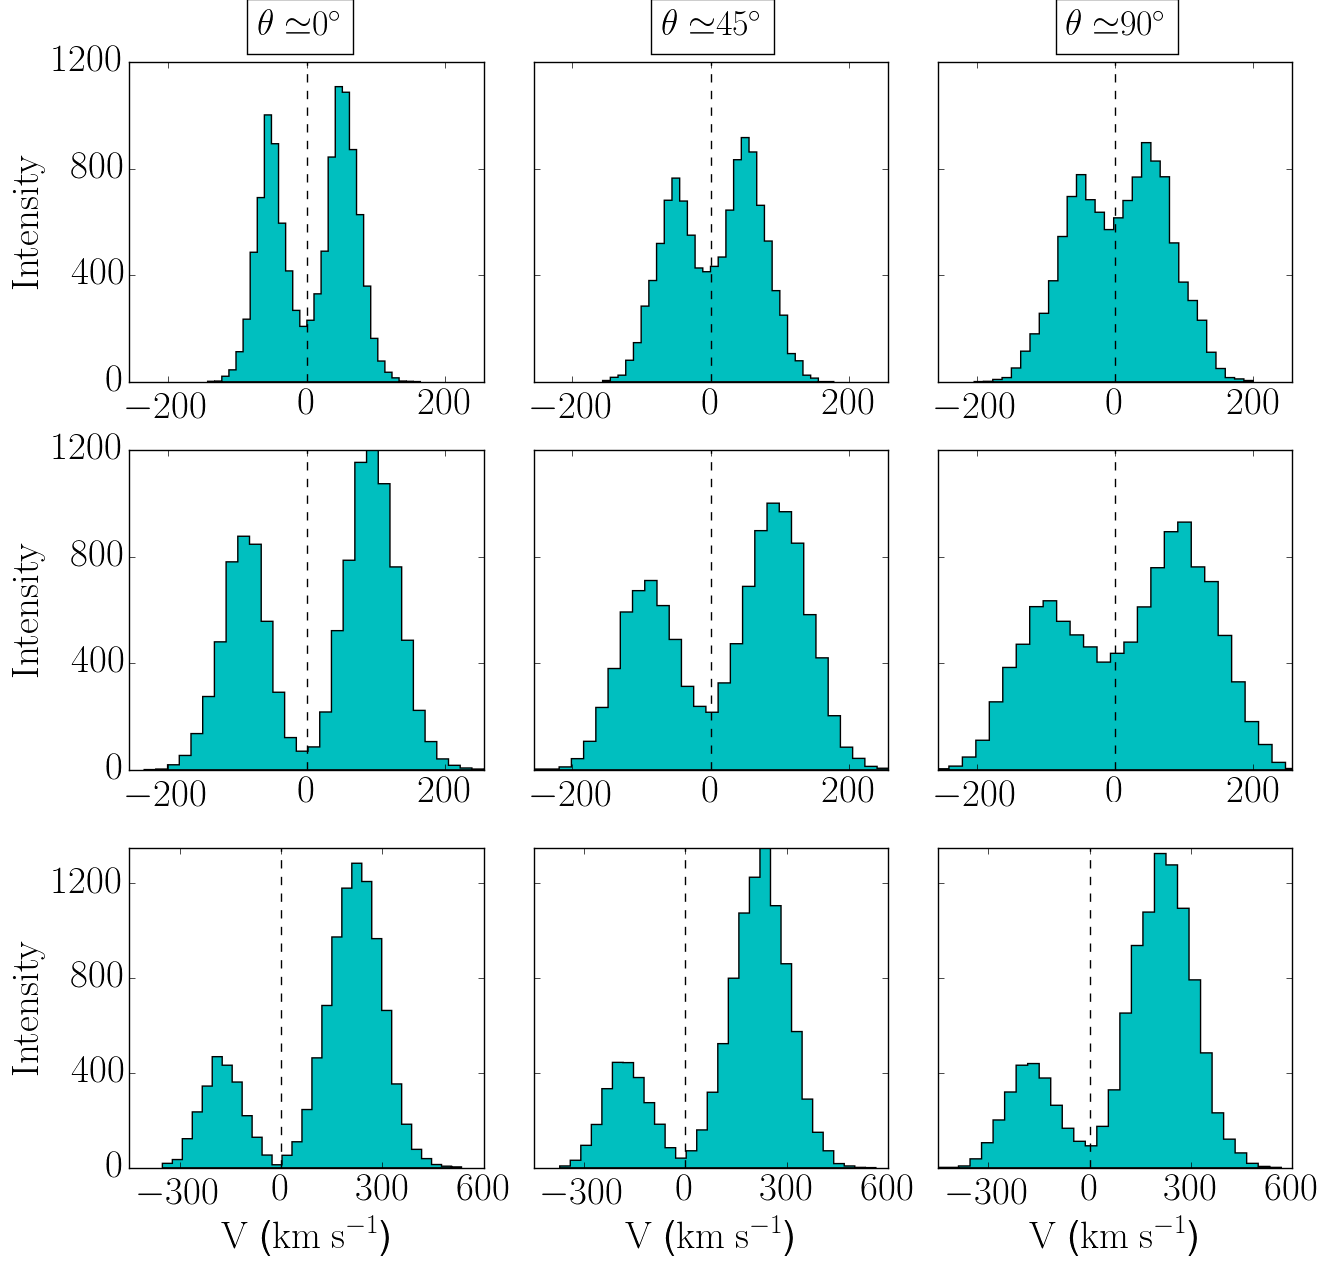
\includegraphics[width=0.5\textwidth]{./figures/angles}
	\end{center}
	\caption{\textbf{\lya profile for different $\theta$.} For tauh$=10^5$, vrot$=50$ \kms and vout$=20$ \kms. For tauh$=10^6$, vrot$=100$ \kms and vout$=5$ \kms. For tauh$=10^7$, vrot$=100$ \kms and vout$=15$ \kms. The intensity is in arbitrary units.
		\label{fig:angles}}
\end{figure}

From Fig. \ref{fig:angles} it is clear that the intensity of the valley between the two peaks increases along with $\theta$. This causes an intensity decrease in the rest of the frequencies, thus a broadening of the line. The asymmetry also changes with the viewing angle.\\


\subsection{Morphology of \lya line}

To summarize, the influence of the 4 parameters on the \lya morphology is the following: 

\begin{itemize}
	\item tauh induces a redshift. Increasing the optical depth separates the line of the zero velocity line. \\
	\item vout decreases the right peak's intensity. Higher vout makes the left peak smaller until it merges with the right one. \\
	\item vrot broadens the line and decreases the maximum intensity. Higher vrot implies a flatter spectrum. This effect has not been deeply studied in literature. Only Garavito et al. \cite{Garavito14} has simulated its effect. Our results are consistent with their conclusions.
	\item $\theta$ increases the central valley of the line. Higher $\theta$ makes more emission at \lya natural frequency. \\ 
\end{itemize}

\subsection{Doppler shift by rotation}

The rotation effect induces a Doppler shift in frequency and displaces the only-outflow spectra. As seen in Fig. \ref{fig:rotation_doppler_outflow} rotation takes the resulting spectrum with vrot$=0$ and displaces it from its central location. Then it weights the lines and they all merge into the resulting red \lya line.\\

\begin{figure}[h!]
	\begin{center}
		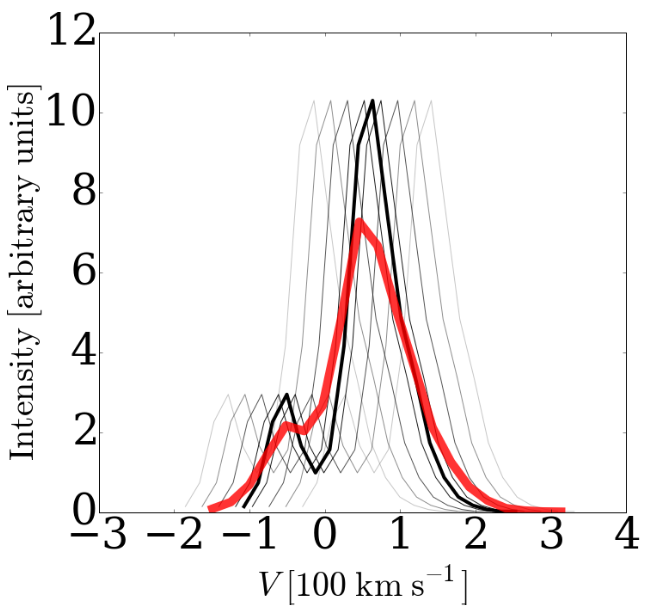
\includegraphics[width=0.3\textwidth]{./figures/rotation_doppler_outflow}
	\end{center}
	\caption{\textbf{Rotations induces a Doppler shift of the only-outflow spectra:} Each of the black lines is then weighted to obtain the red line.
		\label{fig:rotation_doppler_outflow}}
\end{figure}

PONER GRAFICA REAL...\\

\section{Observational Implications}
\label{sec:observationalimplications}

Among the observational implications that this paper has over observations we select three principal ones. First, the rotational effects of the galaxy should be clearly detected and characterized by MUSE's high resolution data. The Doppler redshift is already visible in other observations, such as the one seen in Fig. 7 of Prescott et al. \cite{Prescott14}.\\

Second, the central ($V=0$) emission of the spectra seen in the results is a consequence of the viewing angle of the galaxy and can be controlled by it. This means that the reason is not necessary that radiation is escaping without scattering, as several authors have suggested (CITAS...).\\

Finally, all the spectra produced from this new LAE model is roughly consistent with observations. The consideration of adding the new rotation parameter to the standard only-outflow model found in literature is reasonable and very powerful. vrot and its consequent viewing angle $\theta$ can modify the morphology of the \lya line in new different ways by keeping the model simplified.\\

\section{Conclusions}
\label{sec:conclusions}

In this paper, the objective was to analyze and measure the influence of galaxy rotation and outflows on the \lya line. The motivation for this is to be able to obtain physical information of a LAE by just looking at its \lya profile. In order to accomplish this objective, we propose a new model of a LAE consisting of a sphere of Hydrogen atoms that expands radially and rotates as a solid body. A modified version of the program CLARA \cite{CLARA} is used to set the conditions and emulate the radiative transfer process inside the galaxy. \\

The conclusions obtained from this work are: 

\begin{itemize}
	\item The outgoing spectra depend on the angle an external observer is viewing the galaxy from. The closer it is to the equator of the galaxy, the higher the central valley of the frequency distribution. 
	
	\item The effects of vrot, vout and tauh are consistent with the different authors that have used them. vrot broadens the \lya line. vout increases the peaks asymmetry and tauh induces a redshift around the zero velocity.
	
	\item Rotations induces a Doppler shift in frequency of the only-outflow spectra.
	
	\item The final spectra obtained are roughly consistent with LAEs observations. \\ 

\end{itemize}

\subsection{Future work}

For future work regarding the model, we would like to implement a differential rotation for the LAE instead of solid body. Regarding result analysis, we would like to compare against observations in two ways. Firstly by using the kinematic observation obtained from newly observed LAEs. We could do a consistency check between their real spectra and the simulated one that our model would produce with the respective parameters. Secondly we would like to take a specific observed spectrum and fit it using MCMC in order to predict ranges for its parameters. \\

\subsection{Reproducibility}

All of this work is available online and free to use to anyone. The data, source code and instructions to replicate this paper's results are in the GitHub repository:  \texttt{github.com/astroandes/CLARA\_RotationOutflows}. \\


\section*{Acknowledgments}
The authors would like to acknowledge the high performance computational cluster (HPC) hosted by Universidad de los Andes, where we ran the simulations for CLARA. \\

We would also like to acknowledge the participants of the meeting \textit{Escape of Lyman radiation from galactic labyrinths} at Crete, Greece, for their valuable comments on this work, specially to Max Gronke and Christian Herenz. \\


%------------------------REFERENCES----------------------------
